\section{Característiques d'una funció}

\subsection{Domini i recorregut}

El conjunt de tots els valors reals de la variable independent que tenen per imatge un nombre real constitueixen el \textbf{domini} de la funció, expressat com $D_f$. El conjunt de totes les imatges reals de la funció és el \textbf{recorregut} o \textbf{rang} de la funció.

\begin{table}[!htbp]
\centering
\renewcommand{\arraystretch}{1.75}
\begin{tabular}{lc}
\toprule
Funció & Domini ($D_f$) \\
\midrule
Polinòmica $P(x)$ & $\mathbb{R}$ \\
Racional $\displaystyle \dfrac{P(x)}{Q(x)}$ & $\mathbb{R} - \{x : Q(x) = 0\}$ \\
Arrel $\sqrt[n]{P(x)}$, $n$ parell & $\mathbb{R} - \{x : P(x) < 0\}$ \\
Arrel $\sqrt[n]{P(x)}$, $n$ imparell & $\mathbb{R}$ \\
Logarítmica $\log(f(x))$ & $\mathbb{R} - \{x : f(x) \le 0\}$ \\
Exponencial $e^{f(x)}$ & $D(f)$ \\
\bottomrule
\end{tabular}
\caption{domini de les principals famílies de funcions.}
\end{table}

\subsection{Simetries}

\begin{itemize}
\item Una funció és \textbf{parella} si $f(-x) = f(x)$. La seva gràfica és simètrica respecte a l'eix d'ordenades.
\item Una funció és \textbf{imparella} si $f(-x) = -f(x)$. La seva gràfica és simètrica respecte de l'origen.
\end{itemize}

\subsection{Punts de tall amb els eixos de coordenades}

\begin{itemize}
\item Tall amb l'eix $X$ $(-, 0)$: quan $f(x) = 0$.
\item Tall amb l'eix $Y$ $(0, -)$: quan $x = 0$, és a dir, $f(0)$.
\end{itemize}

\section{Asímptotes}

Definim una \textbf{asímptota} com aquella recta límit de les rectes tangents a la gràfica de la funció quan el punt de tangència tendeix a infinit. La distància entre l'asímptota i la gràfica de la funció tendeix a zero. Hi ha tres tipus d'asímptotes:

\begin{figure}[!htbp]
\centering
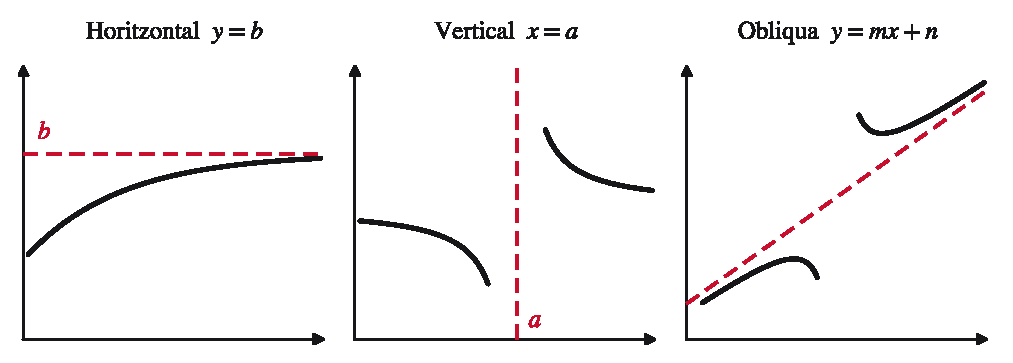
\includegraphics[width=440pt]{fig/m03_f11.pdf}
\caption{Els tres tipus d'asímptotes: horitzontal ($y = b$), vertical ($x = a$) i obliqua ($y = mx + n$).}
\end{figure}

\subsection{Asímptota vertical}

Si $f(x)$ té una discontinuïtat asimptòtica en el punt $x = a$, la recta $x = a$ és una asímptota vertical de la funció:

\begin{equation*}
\lim_{x\to a} f(x) = \infty
\end{equation*}

\subsection{Asímptota horitzontal}

Si $\displaystyle\lim_{x\to\pm\infty} f(x) = b$, la recta $y = b$ és una asímptota horitzontal. En funcions racionals $P(x)/Q(x)$:

\begin{itemize}
\item Si $\operatorname{gr}(P) > \operatorname{gr}(Q)$: no hi ha asímptota horitzontal.
\item Si $\operatorname{gr}(P) = \operatorname{gr}(Q)$: $y = \dfrac{\text{coef. principal de } P}{\text{coef. principal de } Q}$ és l'A.H.
\item Si $\operatorname{gr}(P) < \operatorname{gr}(Q)$: $y = 0$ és l'asímptota horitzontal.
\end{itemize}

\subsection{Asímptota obliqua}

L'asímptota obliqua té la forma $y = mx + n$, on:

\begin{equation*}
m = \lim_{x\to\pm\infty} \frac{f(x)}{x}, \qquad n = \lim_{x\to\pm\infty}\bigl[f(x) - mx\bigr]
\end{equation*}

En funcions racionals, existeix asímptota obliqua quan el grau del numerador supera en exactament 1 el grau del denominador (per exemple, $\dfrac{x^2+1}{x+3}$, graus 2 i 1).

\section{Optimització}

Els problemes d'\textbf{optimització} són aquells en els quals es busca el valor que fa màxima o mínima una determinada funció que correspon a la matematització d'una situació pràctica.

Per analitzar una funció, s'utilitza el signe de la derivada primera $f'(x)$ sobre la recta real, identificant els punts clau (zeros de $f'$) i determinant si corresponen a màxims, mínims o punts d'inflexió de tangent horitzontal.

\section{Complement: optimització --- mètode i exemples}

\subsection{Mètode general}

\begin{enumerate}
\item Identificar la quantitat a maximitzar o minimitzar i expressar-la com a funció $f(x)$.
\item Determinar el domini de $f$: restriccions físiques o geomètriques del problema.
\item Derivar $f'(x)$ i resoldre $f'(x) = 0$ per trobar els \textbf{punts crítics}.
\item Classificar cada punt crític:
\begin{itemize}
\item Si $f''(x_0) > 0 \Rightarrow$ mínim local.
\item Si $f''(x_0) < 0 \Rightarrow$ màxim local.
\item Comparar també els valors als extrems del domini.
\end{itemize}
\item Respondre amb les unitats correctes.
\end{enumerate}

\subsection{Exemple 1 --- Àrea màxima d'un rectangle}

Un agricultor té $80$ m de tanca per delimitar un rectangle. Quines dimensions fan l'àrea màxima?

Sigui $x$ l'amplada i $y$ l'alçada. Restricció: $2x + 2y = 80 \Rightarrow y = 40 - x$.

\begin{equation*}
A(x) = x\,(40 - x) = 40x - x^2, \qquad x \in (0, 40)
\end{equation*}

\begin{equation*}
A'(x) = 40 - 2x = 0 \Rightarrow x = 20
\end{equation*}

$A''(x) = -2 < 0 \Rightarrow$ màxim. $\;A(20) = 20\cdot 20 = 400\ \text{m}^2$.

La forma òptima és un \textbf{quadrat de $20\times 20$ m}.

\subsection{Exemple 2 --- Volum màxim d'una caixa}

D'una làmina quadrada de costat $12$ cm es retallen quadrats iguals de costat $x$ als quatre cantons i es plega. Quina $x$ maximitza el volum?

\begin{equation*}
V(x) = x\,(12 - 2x)^2, \qquad x \in (0, 6)
\end{equation*}

\begin{equation*}
V'(x) = (12-2x)^2 + x\cdot 2(12-2x)(-2) = (12-2x)\bigl[(12-2x) - 4x\bigr] = (12-2x)(12-6x)
\end{equation*}

$V'(x) = 0 \Rightarrow x = 6$ (extrem) o $x = 2$.

$V(2) = 2\cdot(8)^2 = 128\ \text{cm}^3 \Rightarrow$ \textbf{màxim}.

\subsection{Exemple 3 --- Cost mínim: una llauna cilíndrica}

Es vol fabricar una llauna cilíndrica d'un litre ($1000\ \text{cm}^3$). Quines dimensions minimitzen el material (àrea total)?

Radi $r$ i alçada $h$. Restricció del volum: $\pi r^2 h = 1000 \Rightarrow h = \dfrac{1000}{\pi r^2}$.

\begin{equation*}
A(r) = 2\pi r^2 + 2\pi r h = 2\pi r^2 + \frac{2000}{r}, \qquad r > 0
\end{equation*}

\begin{equation*}
A'(r) = 4\pi r - \frac{2000}{r^2} = 0 \;\Rightarrow\; r^3 = \frac{500}{\pi} \;\Rightarrow\; r = \sqrt[3]{\frac{500}{\pi}} \approx 5{,}42\ \text{cm}
\end{equation*}

$A''(r) = 4\pi + \dfrac{4000}{r^3} > 0 \Rightarrow$ \textbf{mínim}. Llavors $h = \dfrac{1000}{\pi r^2} \approx 10{,}84\ \text{cm}$, és a dir, $h = 2r$: la llauna òptima té l'alçada igual al diàmetre.

\section{Complement: estudi i representació gràfica d'una funció}

Representar una funció significa reunir tota la informació anterior en un dibuix. El \textbf{mètode} és sempre el mateix:

\begin{enumerate}
\item \textbf{Domini} de $f$ (quocients, arrels, logaritmes).
\item \textbf{Simetries:} parella si $f(-x)=f(x)$ (simètrica respecte de l'eix $OY$); imparella si $f(-x)=-f(x)$ (simètrica respecte de l'origen).
\item \textbf{Punts de tall:} amb l'eix $OY$, $f(0)$; amb l'eix $OX$, $f(x)=0$.
\item \textbf{Asímptotes:} verticals (punts fora del domini), horitzontals i obliqües (límits a $\pm\infty$).
\item \textbf{Monotonia i extrems:} signe de $f'$; punts crítics $f'(x)=0$.
\item \textbf{Curvatura i inflexions:} signe de $f''$; punts on $f''(x)=0$.
\item \textbf{Taula de valors} amb tots els punts singulars, i dibuix de la gràfica amb una corba suau.
\end{enumerate}

\subsection{Exemple 1 --- Un polinomi: $f(x)=x^3-3x$}

\begin{itemize}
\item \textbf{Domini:} $\mathbb{R}$. \textbf{Simetria:} $f(-x)=-f(x)$, imparella.
\item \textbf{Talls:} $f(0)=0$; $x^3-3x=x(x^2-3)=0 \Rightarrow x=0,\ x=\pm\sqrt3$.
\item \textbf{Asímptotes:} cap (és un polinomi).
\item \textbf{Monotonia:} $f'(x)=3x^2-3=3(x-1)(x+1)$, s'anul\textperiodcentered{}la en $x=\pm1$.
\end{itemize}

\begin{table}[!htbp]
\centering
\renewcommand{\arraystretch}{1.3}
\begin{tabular}{lccc}
\toprule
Interval & $(-\infty,-1)$ & $(-1,1)$ & $(1,+\infty)$ \\
\midrule
Signe de $f'$ & $+$ & $-$ & $+$ \\
$f$ & creix & decreix & creix \\
\bottomrule
\end{tabular}
\end{table}

Màxim relatiu $(-1,\,2)$ i mínim relatiu $(1,\,-2)$.

\begin{itemize}
\item \textbf{Curvatura:} $f''(x)=6x$: còncava ($\cap$) per a $x<0$, convexa ($\cup$) per a $x>0$. Inflexió en $(0,\,0)$.
\end{itemize}

\begin{figure}[!htbp]
\centering
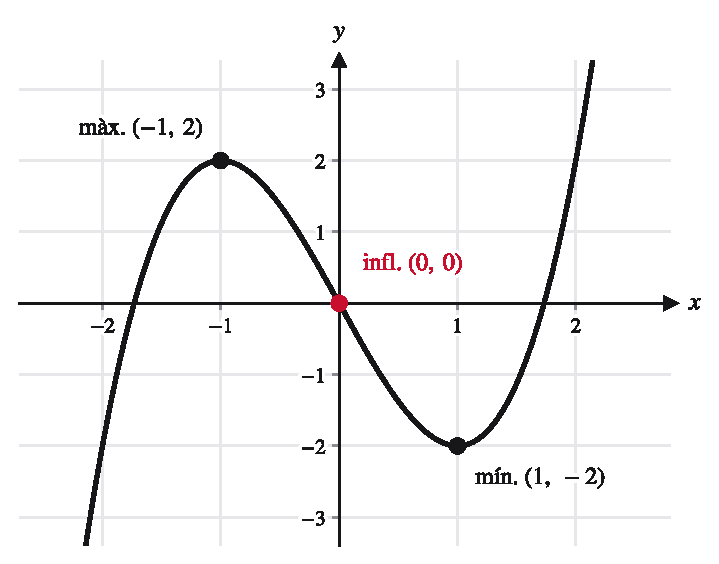
\includegraphics[width=345pt]{fig/m03_f31.pdf}
\caption{Gràfica de $f(x)=x^3-3x$ amb el màxim, el mínim i el punt d'inflexió.}
\end{figure}

\subsection{Exemple 2 --- Una funció racional: $f(x)=\dfrac{x^2}{x-1}$}

\begin{itemize}
\item \textbf{Domini:} $\mathbb{R}\setminus\{1\}$. \textbf{Simetria:} cap.
\item \textbf{Talls:} $f(0)=0$ i $x^2=0\Rightarrow x=0$ (només l'origen).
\item \textbf{Asímptota vertical:} $x=1$. $\displaystyle\lim_{x\to1^+}f=+\infty$ i $\displaystyle\lim_{x\to1^-}f=-\infty$.
\item \textbf{Asímptota obliqua:} $m=\displaystyle\lim_{x\to\infty}\frac{f(x)}{x}=1$ i $n=\displaystyle\lim_{x\to\infty}\left(\frac{x^2}{x-1}-x\right)=\lim\frac{x}{x-1}=1$. Per tant $y=x+1$.
\item \textbf{Monotonia:} $f'(x)=\dfrac{2x(x-1)-x^2}{(x-1)^2}=\dfrac{x(x-2)}{(x-1)^2}$, s'anul\textperiodcentered{}la en $x=0$ i $x=2$.
\end{itemize}

\begin{table}[!htbp]
\centering
\renewcommand{\arraystretch}{1.3}
\begin{tabular}{lcccc}
\toprule
Interval & $(-\infty,0)$ & $(0,1)$ & $(1,2)$ & $(2,+\infty)$ \\
\midrule
Signe de $f'$ & $+$ & $-$ & $-$ & $+$ \\
$f$ & creix & decreix & decreix & creix \\
\bottomrule
\end{tabular}
\end{table}

Màxim relatiu $(0,\,0)$ i mínim relatiu $(2,\,4)$.

\begin{itemize}
\item \textbf{Curvatura:} $f''(x)=\dfrac{2}{(x-1)^3}$: còncava per a $x<1$ i convexa per a $x>1$. No hi ha punts d'inflexió ($f''\neq0$ sempre).
\end{itemize}

\begin{figure}[!htbp]
\centering
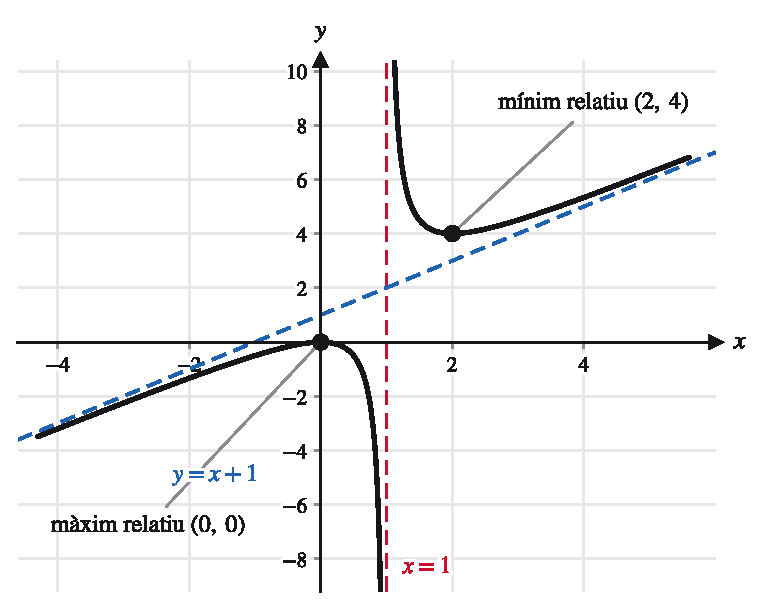
\includegraphics[width=367pt]{fig/m03_f32.pdf}
\caption{Gràfica de $f(x)=\dfrac{x^2}{x-1}$ amb l'asímptota vertical $x=1$ (vermell) i l'obliqua $y=x+1$ (blau).}
\end{figure}

\subsection{Exemple 3 --- Amb exponencial: $f(x)=x\,e^{-x}$}

\begin{itemize}
\item \textbf{Domini:} $\mathbb{R}$. \textbf{Talls:} $f(0)=0$ i $x\,e^{-x}=0\Rightarrow x=0$.
\item \textbf{Límits:} $\displaystyle\lim_{x\to+\infty}xe^{-x}=0$ (l'exponencial guanya): asímptota horitzontal $y=0$. Per a $x\to-\infty$, $f\to-\infty$ sense asímptota.
\item \textbf{Monotonia:} $f'(x)=e^{-x}(1-x)$, s'anul\textperiodcentered{}la en $x=1$. Creix per a $x<1$ i decreix per a $x>1$: màxim en $\left(1,\,\dfrac1e\right)$.
\item \textbf{Curvatura:} $f''(x)=e^{-x}(x-2)$: còncava per a $x<2$, convexa per a $x>2$. Inflexió en $\left(2,\,\dfrac{2}{e^2}\right)$.
\end{itemize}

\begin{figure}[!htbp]
\centering
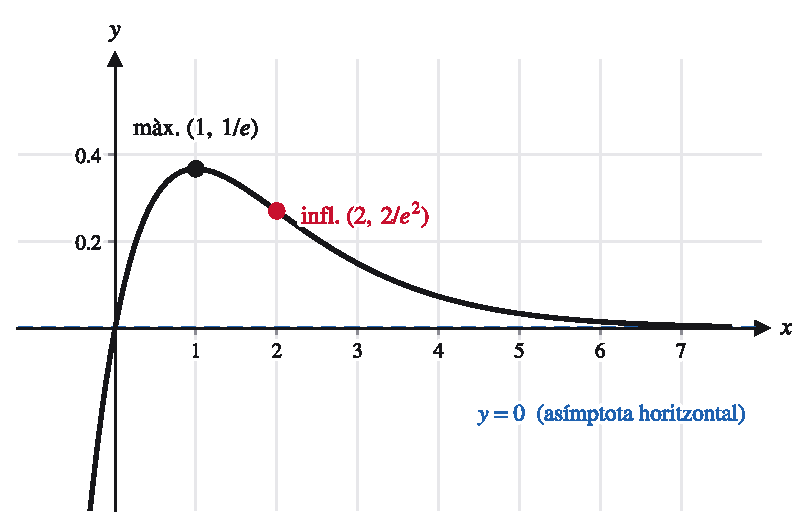
\includegraphics[width=389pt]{fig/m03_f33.pdf}
\caption{Gràfica de $f(x)=x\,e^{-x}$: màxim en $x=1$, inflexió en $x=2$ i asímptota horitzontal $y=0$ cap a $+\infty$.}
\end{figure}

\section{Complement: esquema per a l'estudi complet d'una funció}

Per representar una funció $y=f(x)$ s'aconsella seguir sempre aquest ordre:

\begin{enumerate}
\item \textbf{Domini} i, si cal, recorregut.
\item \textbf{Simetries:} parella ($f(-x)=f(x)$), imparella ($f(-x)=-f(x)$) i periodicitat.
\item \textbf{Punts de tall} amb els eixos: $f(0)$ i les solucions de $f(x)=0$.
\item \textbf{Asímptotes:} verticals (en els punts on el límit és infinit), horitzontals i obliqües.
\item \textbf{Primera derivada:} signe de $f'$, intervals de creixement i decreixement, extrems relatius.
\item \textbf{Segona derivada:} signe de $f''$, intervals de concavitat i punts d'inflexió.
\item \textbf{Taula resum} amb tots els punts notables i \textbf{gràfica} final.
\end{enumerate}

\section{Complement: més problemes d'optimització}

\emph{Exemple 4 --- Punt d'una corba més proper a un punt donat:} Trobem el punt de la paràbola $y=x^2$ més proper a $A=\bigl(0,\tfrac32\bigr)$. Es minimitza el quadrat de la distància (el mateix punt minimitza la distància i s'evita l'arrel):

\begin{equation*}
d^2(x)=x^2+\Bigl(x^2-\frac32\Bigr)^2=x^4-2x^2+\frac94.
\end{equation*}

Aleshores $(d^2)'=4x^3-4x=4x(x-1)(x+1)=0\Rightarrow x=0,\pm1$. Com que $d^2(0)=\tfrac94$ i $d^2(\pm1)=\tfrac54$, els mínims són els punts $(\pm1,1)$, a distància $d=\dfrac{\sqrt5}{2}\approx1{,}12$. ($x=0$ és un màxim relatiu.)

\emph{Exemple 5 --- Plantilla amb talls:} Per construir la caixa de l'exemple 2 es retallen quadrats de costat $x$ a les quatre cantonades de la làmina de 12 cm. La figura mostra la plantilla i la caixa resultant.

\begin{figure}[!htbp]
\centering
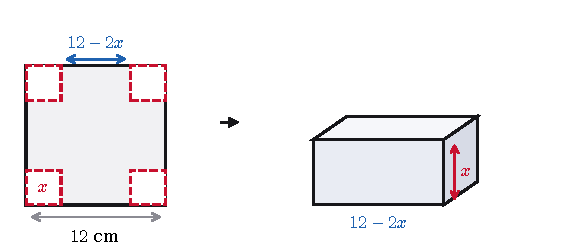
\includegraphics[width=278pt]{fig/x03_box_net.pdf}
\caption{Plantilla de la caixa: es retallen quatre quadrats de costat $x$ i es pleguen els laterals. Base $(12-2x)\times(12-2x)$ i alçada $x$.}
\end{figure}

\emph{Exemple 6 --- Rectangle inscrit en una semicircumferència:} Quin és el rectangle d'àrea màxima inscrit en una semicircumferència de radi $R$? Si el vèrtex és $(x,\sqrt{R^2-x^2})$, l'àrea és $A(x)=2x\sqrt{R^2-x^2}$. Derivant, $A'(x)=\dfrac{2(R^2-2x^2)}{\sqrt{R^2-x^2}}=0\Rightarrow x=\dfrac{R}{\sqrt2}$. Les dimensions són $R\sqrt2\times\dfrac{R}{\sqrt2}$ i l'àrea màxima val $R^2$.

\section{Complement: un altre estudi de funció --- $f(x)=\dfrac{\ln x}{x}$}

\begin{itemize}
\item \textbf{Domini:} $(0,+\infty)$. No té simetria.
\item \textbf{Talls:} amb $OX$ en $\ln x=0\Rightarrow x=1$, punt $(1,0)$. No talla $OY$.
\item \textbf{Asímptotes:} $\displaystyle\lim_{x\to0^{+}}\frac{\ln x}{x}=-\infty$: vertical $x=0$. $\displaystyle\lim_{x\to+\infty}\frac{\ln x}{x}=0$ (Hôpital): horitzontal $y=0$ (per la dreta).
\item \textbf{Primera derivada:} $f'(x)=\dfrac{1-\ln x}{x^2}$. S'anul\textperiodcentered{}la en $x=e$; $f'>0$ si $x<e$ i $f'<0$ si $x>e$. Màxim relatiu (i absolut) en $\bigl(e,\tfrac1e\bigr)\approx(2{,}72;\,0{,}37)$.
\item \textbf{Segona derivada:} $f''(x)=\dfrac{2\ln x-3}{x^3}$. S'anul\textperiodcentered{}la en $x=e^{3/2}\approx4{,}48$: $f''<0$ abans (convexa $\cap$) i $f''>0$ després (còncava $\cup$). Inflexió en $\bigl(e^{3/2},\tfrac32e^{-3/2}\bigr)\approx(4{,}48;\,0{,}33)$.
\end{itemize}

\begin{table}[!htbp]
\centering
\renewcommand{\arraystretch}{1.3}
\begin{tabular}{lccccc}
\toprule
$x$ & $(0,e)$ & $e$ & $(e,e^{3/2})$ & $e^{3/2}$ & $(e^{3/2},\infty)$ \\
\midrule
$f'$ & $+$ & $0$ & $-$ & $-$ & $-$ \\
$f''$ & $-$ & $-$ & $-$ & $0$ & $+$ \\
$f$ & creix, $\cap$ & màxim & decreix, $\cap$ & inflexió & decreix, $\cup$ \\
\bottomrule
\end{tabular}
\caption{estudi dels signes de $f'$ i $f''$ per a $f(x)=\ln x/x$.}
\end{table}
